\chapter{ビットごとのT-depthを考慮したMCTゲートの分解手法}
本章では,提案手法である,ビットごとのT-depthを考慮したMCTゲートの分解手法について説明する.
\section{ビットごとのT-depth}
本節では,ビットごとのT-depthについて説明する.
ビットごとのT-depthとは,量子ビットごとにT-depthの値を計算したものである.
\par
ビットごとのT-depthの計算方法について説明する.
図~\ref{toffoli_bit}
にToffoliゲートの分解のビットごとのT-depthを示す.
各入力の量子ビットのビットごとのT-depthを$q_{x}, q_{y}, q_{z}$とする.
まず,図~\ref{toffoli_bit}の
左側の$T$ゲート実行後のT-depthは
その入力のビットごとのT-depthに1を足したものとなる.
図~\ref{toffoli_bit}の黒の実線で囲まれたCNOTゲートは,
入力のビットの実行が終わるまで実行できない.
このため,
黒の実線で囲まれたCNOTゲートの実行後の
ビットごとのT-depthは,入力のビットのビットごとのT-depthの最大値,
すなわち$\max\{q_{x}+1, q_{y}+1\}$と考えることができる.
赤の点線で囲まれたCNOTゲートに関しても同様に考えると,
実行後のビットごとのT-depthは,$\max\{q_{x}+1, q_{y}+1, q_{z}+1\}$となる.
このようにして,
Toffoliゲートの左側から順番にビットごとのT-depthを計算すると,
Toffoliゲート実行後のビットごとのT-depthは,$\max\{q_{x},q_{y},q_{z}\}+3$と考えることができる.
\begin{figure}
  \centering
  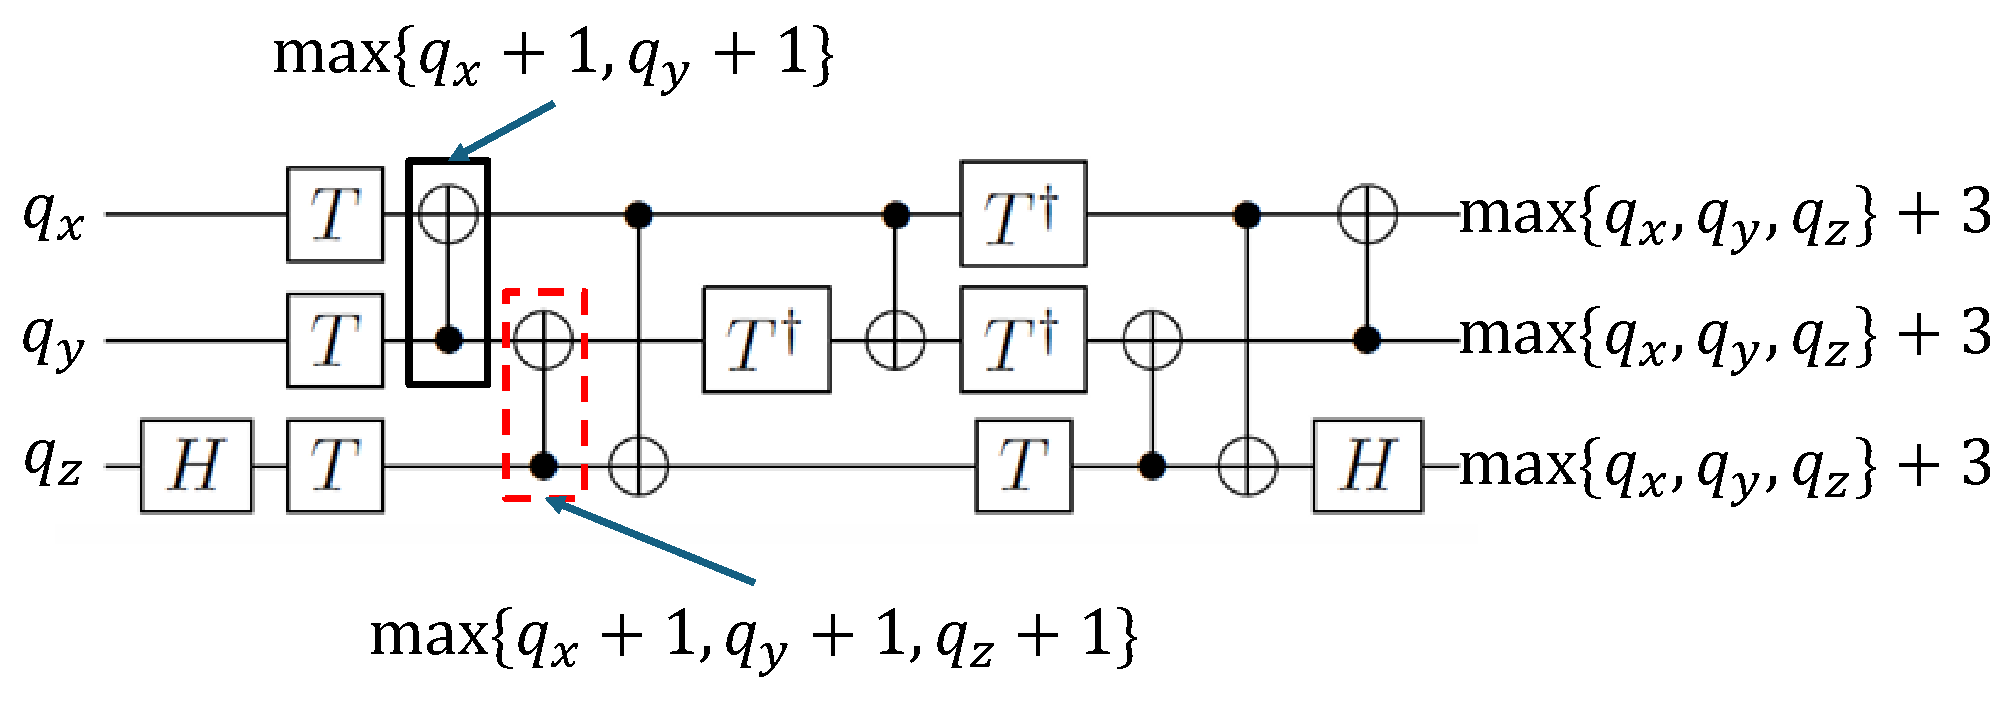
\includegraphics[width=12cm]{img/toffoli_bit.pdf}
  \caption{ToffoliゲートのビットごとのT-depth}
  \label{toffoli_bit}
\end{figure}
\par
ビットごとのT-depthは補助ビットを用いずにClifford+Tに,
分解できるゲートから計算を行うことができる.
表~\ref{tab:gate_tdepth}に補助ビットを用いずに
Clifford+Tに分解できるゲートを実行後のT-depthを示す.
表~\ref{tab:gate_tdepth}に基づき,
回路の左側からビットごとのT-depthを計算することで,
その回路のビットごとのT-depthを求めることができる.
\begin{table}[tbp]
  \centering
  \caption{補助ビットを用いずClifforf+Tに分解できるゲートの実行後のT-depth}
  \label{tab:gate_tdepth}
  \begin{tabular}{c|cc}
    ゲート名                         &使用量子ビット      &実行後のT-depth              \\ \hline
    $T, T^{\dag}$                    &$q_{x}       $      &$q_{x}+1$                    \\
    $H, NOT$                         &$q_{x}$             &$q_{x}$                      \\
    $CNOT$                           &$q_{x}, q_{y}$      &$\max\{q_{x}, q_{y}\}$       \\ 
    \bout{Toffoli}                   &$q_{x}, q_{y}, q_{z}$&$\max\{q_{x},q_{y},q_{z}\}+3$\\
    $CCiZ, CCiZ^{\dag}              $&$q_{x}, q_{y}, q_{z}$&$\max\{q_{x},q_{y},q_{z}\}+2$\\
    $CCi\omega Z, CCi\omega Z^{\dag}$&$q_{x}, q_{y}, q_{z}$&$\max\{q_{x},q_{y},q_{z}\}+1$\\
    $C\omega S, C\omega S^{\dag}$    &$q_{x}, q_{y}       $&$\max\{q_{x},q_{y}\}+1      $\\
  \end{tabular} 
\end{table}
\par
図~\ref{bit_tdepth}に
表~\ref{tab:gate_tdepth}に基づいてビットごとのT-depthを計算した例を示す.
図~\ref{bit_tdepth}の入力のビットごとのT-depthはすべて0とする.
図~\ref{bit_tdepth}の最大のT-depthは12であり,
最小のT-depthは8である.
図~\ref{bit_tdepth}は,
手法~1でコントロールビット数が4のMCTゲートを分解したものの,ビットごとのT-depthを求めたものである.
このようにビットごとのT-depthを計算すると,各ビットのT-depthに差が生じる.
このため,T-depthが小さいビットを優先して使用して,
\rout{MCTゲートを分解することで,}\bout{回路全体の}T-depthを削減することができる.
\begin{figure}
  \centering
  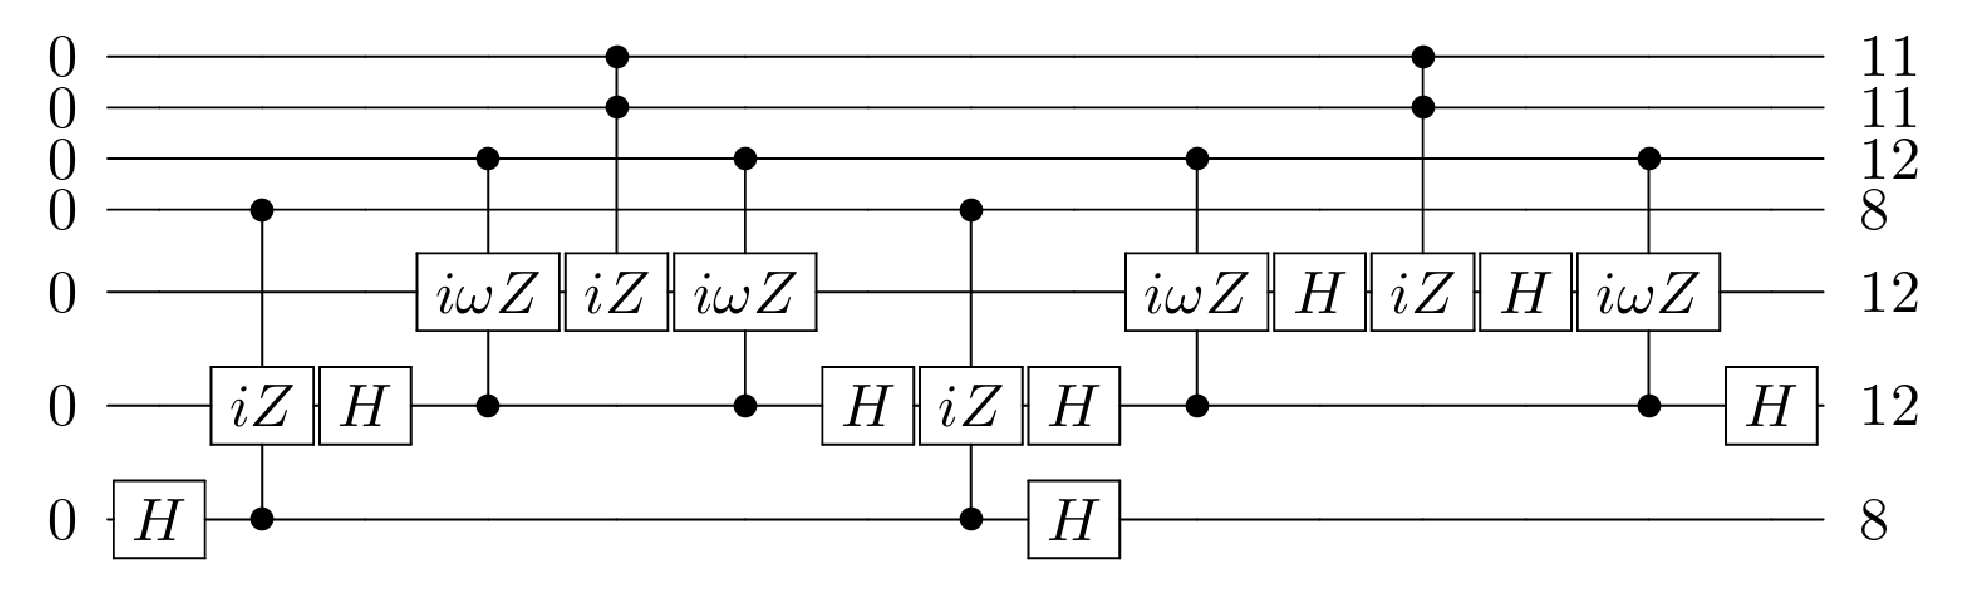
\includegraphics[width=14cm]{img/bit_tdepth.pdf}
  \caption{図~\ref{techmap}の回路のビットごとのT-depth}
  \label{bit_tdepth}
\end{figure}
\par
図~\ref{consider_tdepth}に
コントロールビット数が3個の
MCTゲートをビットごとのT-depthを\rout{考慮して分解した例}を示す.
図~\ref{consider_tdepth}では,入力側の各ビットのT-depthに差が生じている.
そのため,手法~1にビットのT-depthを考慮した分解を適用する場合,
使用するビットのT-depthが小さい順に使用することでT-depthを削減することができる.
図~\ref{bad_consider_tdepth}にビットの選択により分解後の最大のT-depthが悪化する例を示す.
図~\ref{bad_consider_tdepth}の例では,
はじめのゲート$g_{1}$に$q_{4}$のビットを使用した場合,
\bout{後続}のゲートの実行後のT-depthはその値に依存するため,最大のT-depthが20となる.
一方,図~\ref{consider_tdepth}では,
コントロールビットと補助ビットのT-depthが小さい順に使用することで,
分解後のビットのT-depthの最大値を削減している.
\begin{figure}[tbp]
  \centering
  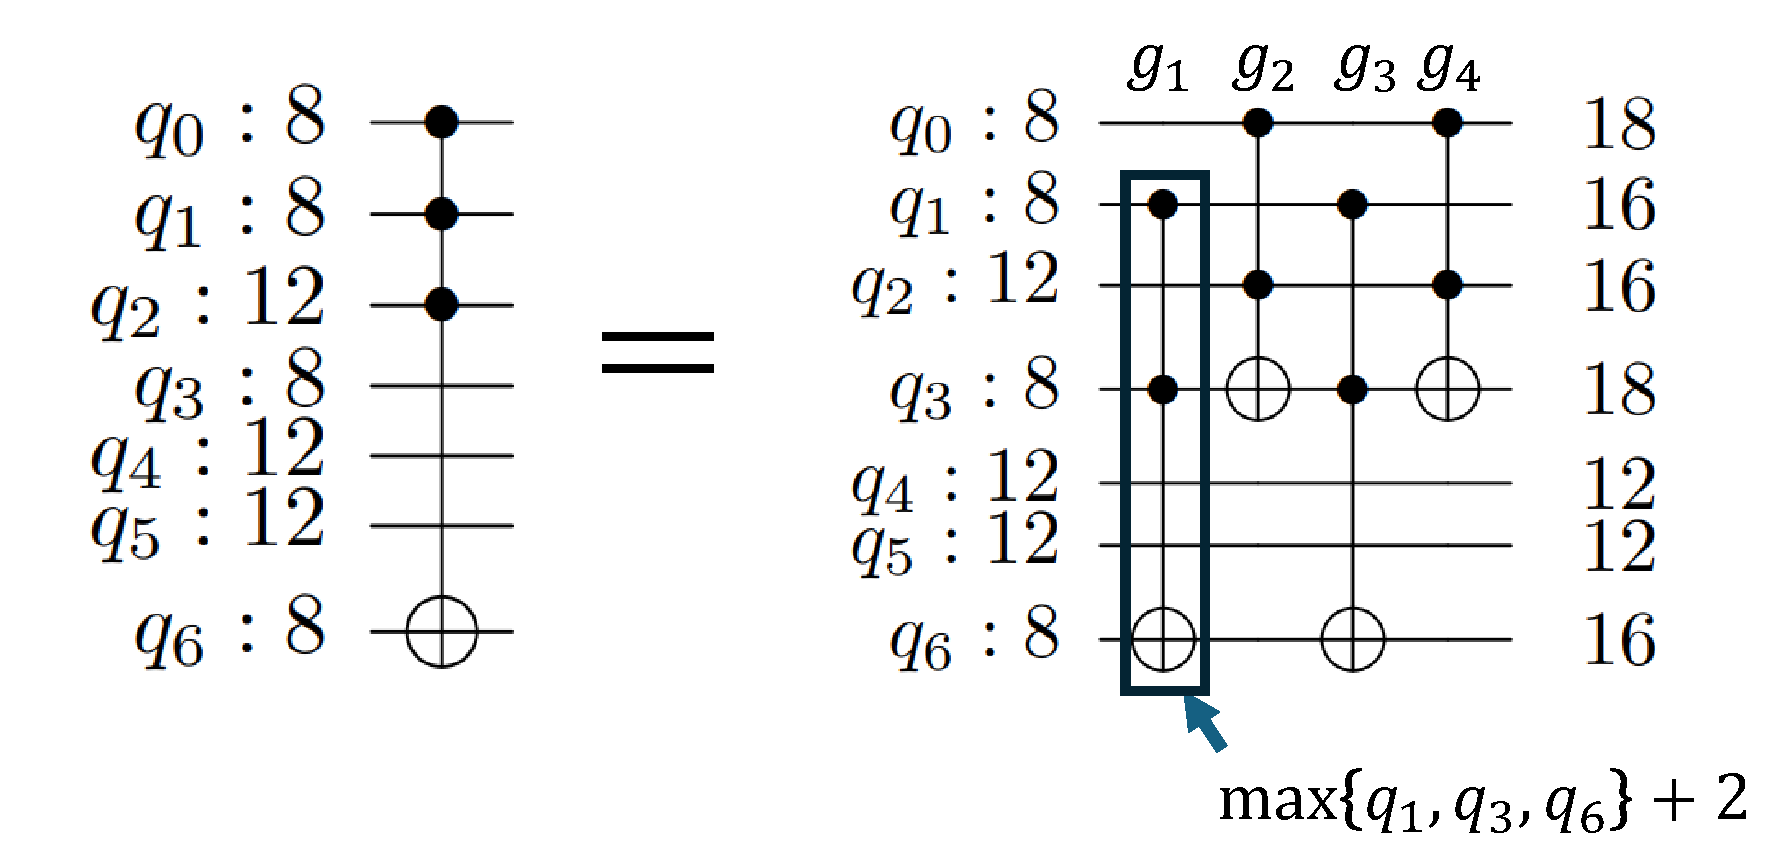
\includegraphics[width=10cm]{img/considering_bit_tdepth.pdf}
  \caption{コントロールビット数が3のMCTゲートをビットごとのT-depthを考慮し分解した例}
  \label{consider_tdepth}
\end{figure}
\begin{figure}[tbp]
  \centering
  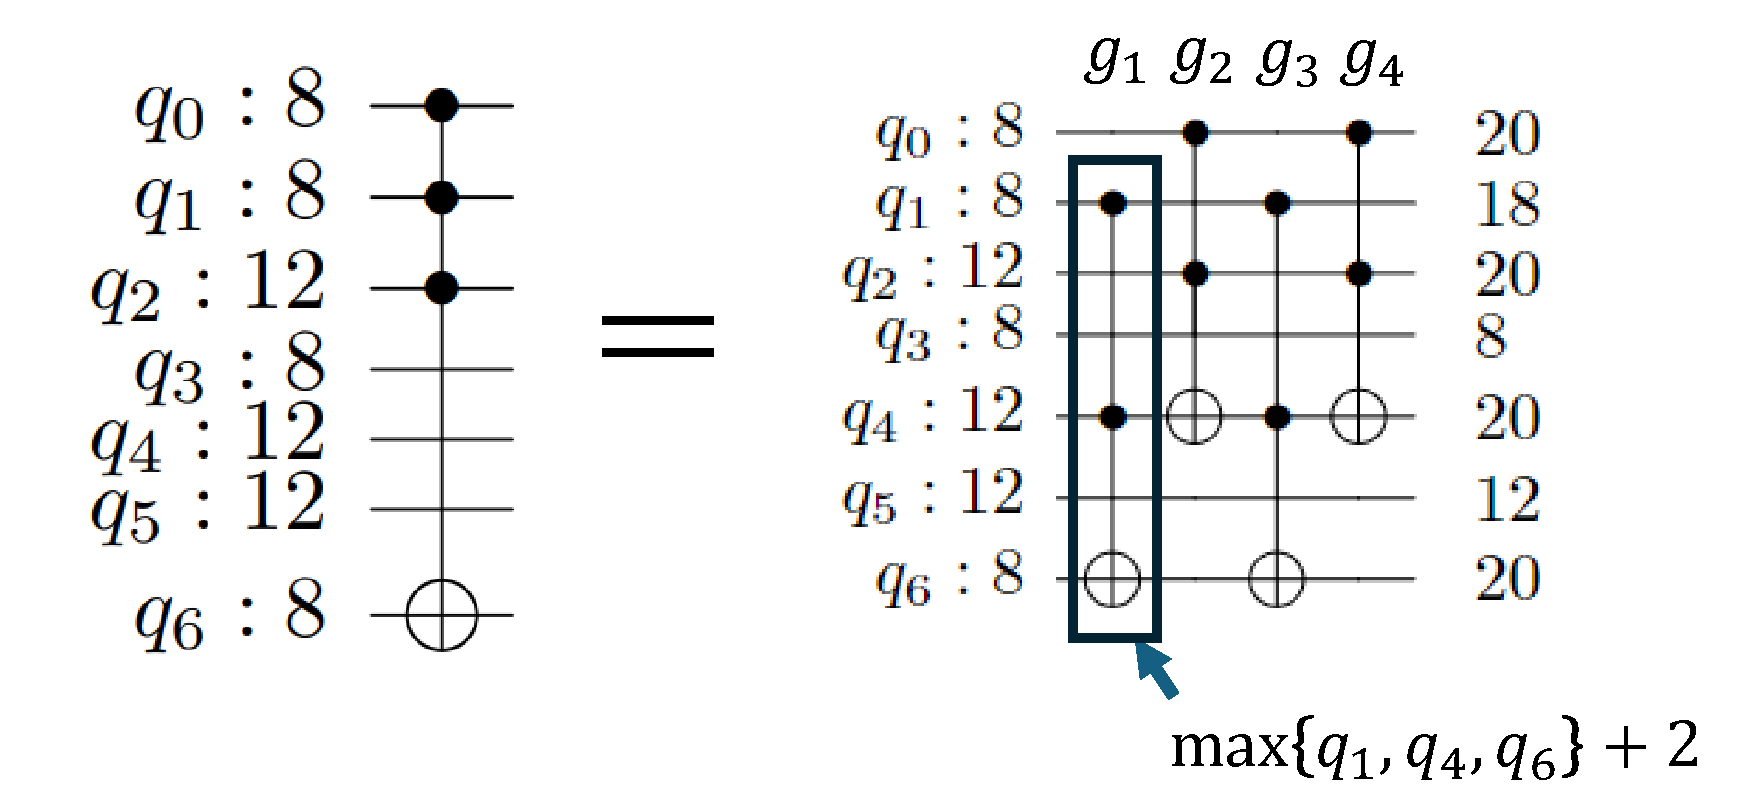
\includegraphics[width=10cm]{img/bad_consider_t-depth.pdf}
  \caption{コントロールビット数が3個のMCTゲートを分解した際に最大のT-depthが悪化する例}
  \label{bad_consider_tdepth}
\end{figure}
\section{ビットごとのT-depthを考慮したMCTゲートの分解}
本節では,
ビットごとのT-depthを考慮した,
MCTゲートの分解について手法1~4に適応\bout{した}方法を説明する.
ここで,分解前のMCTゲートの$c$個のコントロールビットの集合を$C$,
ターゲットビットを$t$とする.
\subsection{手法~1}
本項では,手法~1にビットごとのT-depth
を考慮した分解を適用する方法について説明する.
\par
手法1は,コントロールビットの数が3個以上の
MCTゲートをToffoliゲートに分解した後,
Toffoliゲートを$CCiZ, CCi\omega Z$ゲートに置換する手法である.
そのため,MCTゲートをToffoliゲートに分解する際に,
ゲートの配置が決定する.
\par
MCTゲートをToffoliゲートに分解する際のビットの選択方法について説明する.
図~\ref{barenco}の左から3個分のToffoliゲート\rout{$g_{1},g_{2},g_{3}$}
を構成するビットの配置が決定すれば,
その右側のゲートはこれらのゲートの複製であるため,\bout{MCTゲートの}分解が決定する.
すなわち,
$c-2$個の値が不定の補助ビットを用いてMCTゲートを分解する手法~\cite{barenco1995elementary}では,
$c-1$個のToffoliゲートの配置を決定することで,分解を実現できる.
これらのゲートを構成するビットの決定方法を説明する.
\par
分解前のMCTゲートのコントロールビットを
T-depthが小さい順に並び変えたものを$c_{1},\dots, c_{c}$とする.
分解前のMCTゲートのターゲットビットを$t$とする.
分解後の左から$c-1$個のToffoliゲートを$g_{1},\dots ,g_{c-1}$とする.
$g_{1},\dots, g_{c-1}$の
コントロールビットの集合を$C_{1},\dots, C_{c-1}$とする.
$c-2$個の値が不定の補助ビットをT-depthの小さい順に並び変えたものを,
$a_{1},\dots ,a_{c-2}$とする.
$g_{1},\dots ,g_{c-1}$の構成するビットの決定方法を以下に示す.
\begin{enumerate}[手順1]
  \item $C_{1}\dots, C_{c-2}$に$a_{1},\dots, a_{c-2}$をそれぞれ順番に1つずつ追加する.
  \item $C_{1},\dots ,C_{c-2}$に順番に$c_{1},\dots ,c_{c-2}$を追加する.
  \item $C_{c-1}$に$c_{c-1}, c_{c}$を追加する.
  \item $g_{1}$のターゲットビットを$t$とする.
  \item $g_{2},\dots, g_{c-2}$のターゲットビットをそれぞれ順番\rout{に}$a_{1}, \dots , a_{c-2}$とする.
\end{enumerate}
\par
上記の手順に則り,$g_{1},\dots ,g_{c-1}$を構成するビットを決定した\rout{後,}
式~\ref{eq:toffoli_haiti}の順番に回路の左側からToffoliゲートを配置する.
\begin{equation}\label{eq:toffoli_haiti}
  \{g_{1}, g_{2}, \dots g_{c-1}\}, \{g_{c-2},g_{c-3},\dots g_{1}\}, \{g_{2},g_{3},\dots ,g_{c-1}\}, \{g_{c-2}, g_{c-3}\dots ,g_{2}\}
\end{equation}
最後に,配置したこれらのゲートを手法~1により,$CCiZ, CCi\omega Z$ゲートに置換する.
このように,T-depthの小さいビットを順番に左側のToffoliゲートから配置することで,
T-depthの大きなビットをはじめに使うことを防ぐことができる.
\par
\bout{図~\ref{b2mapping_proposed}はビットごとのT-depthを考慮し,
コントロールビット数が4個のMCTゲートを手法~1で分解した例を示す.
図~\ref{b2mapping_proposed}の左側の分解前のMCTゲートのコントロールビットをT-depthが小さい順に並び変えると,
$C=\{c_{3}, c_{2}, c_{4}, c_{1}\}$である.
値が不定の補助ビットは$a_{1},a_{2}$の順でT-depthが小さい.
まず,$g_{1}, g_{2}, g_{3}$を構成するビットを決定する.
$g_{1}$のコントロールビットを,T-depthが小さい順に選択すると$c_{3}, a_{1}$となり,
ターゲットビットは$t$である.
次に,$g_{2}$のコントロールビットを,
T-depthが小さい順に選択すると,$c_{2}, a_{2}$となり,
ターゲットビットは,$a_{1}$となる.
最後に$g_{3}$のコントロールビットは$c_{4},c_{1}$となり,
ターゲットビットは$a_{2}$となる.
このようにして,$g_{1},g_{2},g_{3}$を構成するビットを決定し,
式~\ref{eq:toffoli_haiti}の順でToffoliゲートを配置する.
配置したToffoliゲートを,手法~1により,$CCiZ, CCi\omega Z$ゲートに置換すると,
図~\ref{b2mapping_proposed}の右側のようになる.この時のT-depthの最大値は,24となる.}
\begin{figure}
  \centering
  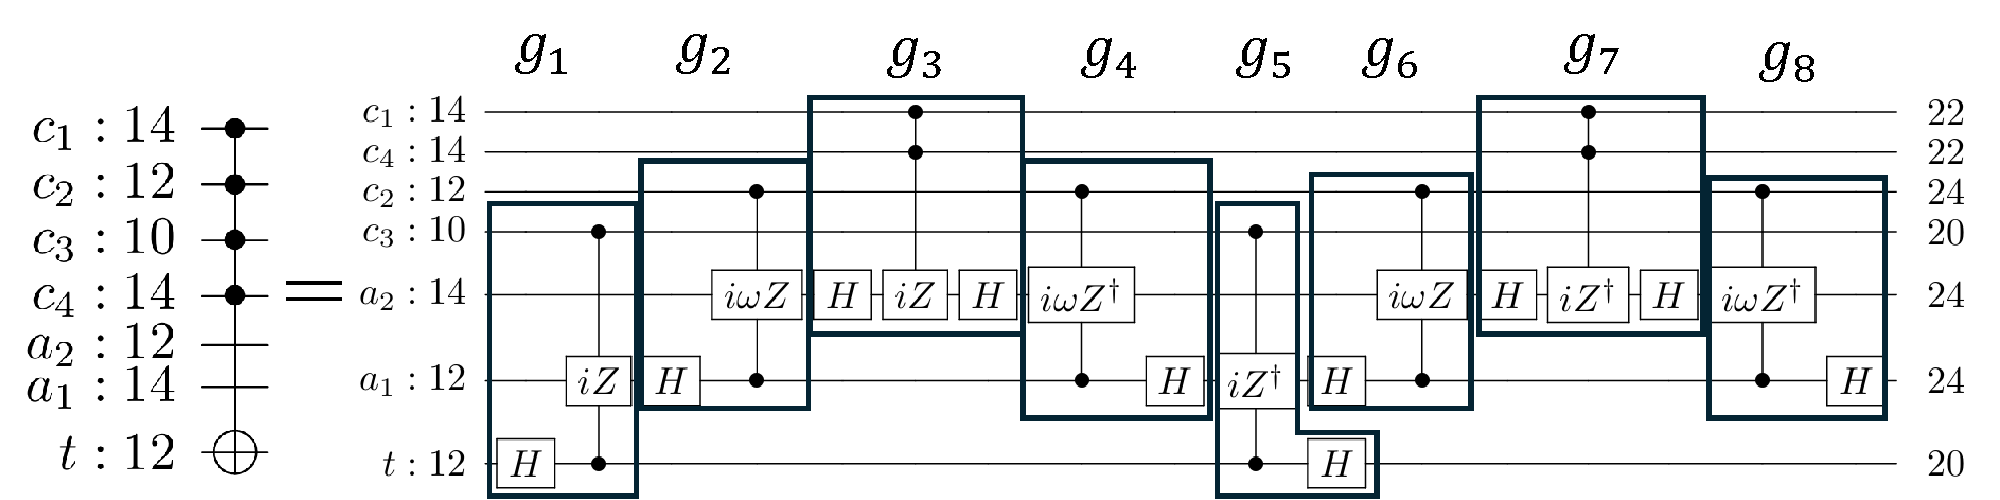
\includegraphics[width=18cm]{img/b2_mapping_proposed.pdf}
  \caption{コントロールビット数が4個のMCTゲートをビットごとのT-depthを考慮し手法1で分解した例}
  \label{b2mapping_proposed}
\end{figure}

\begin{comment}
\begin{algorithm}[tbp]
  \caption{ビットごとのT-depthを考慮した分解}\label{alg:b2map_bit}
  \begin{algorithmic}[1]
    \Require $tdepth\Leftarrow$ 各量子ビットごとのT-depth
    \Require $C\Leftarrow$ 分解するMCTゲートのコントロールビットのリスト
    \Require $t\Leftarrow$ 分解するMCTゲートのターゲットビット
    \Require $D\Leftarrow$ 初期化されていない補助ビットのリスト
    \Ensure $circ$: 分解済みのMCTゲート
    \State $C \Leftarrow$ コントロールビットのリストをT-depthが小さい順にソート
    \State $D \Leftarrow$ 補助ビットのリストをT-depthが小さい順にソート
    \For{$(q,index) \leftarrow $Cの要素とそのindex}
    \If{$i==0$}
      \State 
    \EndIf
    \EndFor
  \end{algorithmic}
\end{algorithm}
\end{comment}
\subsection{手法2}
本項では,ビットごとのT-depthを考慮した分解を手法~2に適用する方法を説明する.
\par
手法~2では,MCTゲートを4つの$C\omega S$ゲートと4つのMCTゲートに分解する.
まず,分解で現れる4つの$C\omega S$ゲートと4つのMCTゲートを構成するビットの決定方法について
説明する.
1つの値が不定のビットを$a$とする.
まず,4つの$C\omega S$ゲートは1つの値が不定の補助ビット$a$をコントロールビットに持ち,
ターゲットビットに$t$をもつ.
次に,分解で現れる4つのMCTゲートは左側から,$g_{1},\dots, g_{4}$とする.
$g_{1}, g_{2}$を構成するビットの決定方法について説明する.
$g_{1}, g_{2}$のコントロールビットの集合を$C_{1}, C_{2}$とする.
分解前のMCTゲートの$c$個のコントロールビットを,
T-depthが小さい順にソートしたものを$c_{1},\dots, c_{c}$とする.
式~\ref{eq:method2bunkatu}の通りに$C_{1}, C_{2}$を決定する.
\begin{equation}\label{eq:method2bunkatu}
  C_{1}=\{c_{1},\dots, c_{\lfloor c/2 \rfloor}\}, C_{2}=\{c_{\lfloor c/2 \rfloor +1},\dots , c_{c}\}
\end{equation}
$g_{1}, g_{2}$のターゲットビットは$a$である.
$g_{3}, g_{4}$についてはそれぞれ,$g_{1}$, $g_{2}$の複製であるため,
これらのゲートと同じビットで構成される.
このようにして,
分解で現れる4つの$C\omega S$ゲートと4つのMCTゲートを構成するビットを決定する.
\par
分解で現れる4つの$C\omega S$ゲートと
4つのMCTゲートを構成するビットを決定した後,
これらのゲートを左側から順番に分解して,ビットごとのT-depthの更新を繰り返す.
Algorithm~\ref{alg:method2_placement_decomp}に従い,これらのゲートを分解,配置する.
このように,左側のゲートから分解することで,
各ゲートをビットごとのT-depthを考慮し,\bout{MCTゲートを}分解できる.
\begin{algorithm}[tbp]
  \caption{ビットごとのT-depthを考慮した手法~2の分解と配置}
  \label{alg:method2_placement_decomp}
  \begin{algorithmic}[1]
    \Require MCTゲート$g_{1},\dots, g_{4}$
    \Require $C\omega S$ゲート
    \Require 各ビット$c_{1},\dots, c_{c}, a, t$とT-depthの対応
    \Ensure 補助ビットを用いずClifford+Tに分解できるゲートで構成される回路$OC$
    \State $g_{i}$のコントロールビットの集合$C_{i}$
    \For{i={1,\dots ,2}}
    \State $OC$に$C\omega S$ゲートを追加,各ビットのT-depthを更新
    \State $C_{(i+1)\% 2}$からT-depthの小さい順にビットを$|C_{i}|-2$個取り出す.
    \State 取り出した$|C_{i}-2|$個のビットを補助ビットとして$g_{i}$をビットごとのT-depthを考慮し手法~1により分解.
    \State $g_{i}$の分解結果を$OC$に追加,各ビットのT-depthを更新
    \EndFor
    \For{i={1,\dots ,2}}
    \State $OC$に$C\omega S$ゲートを追加する.
    \State $OC$に$g_{i}$の分解を逆変換のゲートに置換した上で逆順にしたものを追加する.
    \EndFor
  \end{algorithmic}
\end{algorithm}
\par
\begin{figure}
  \centering
  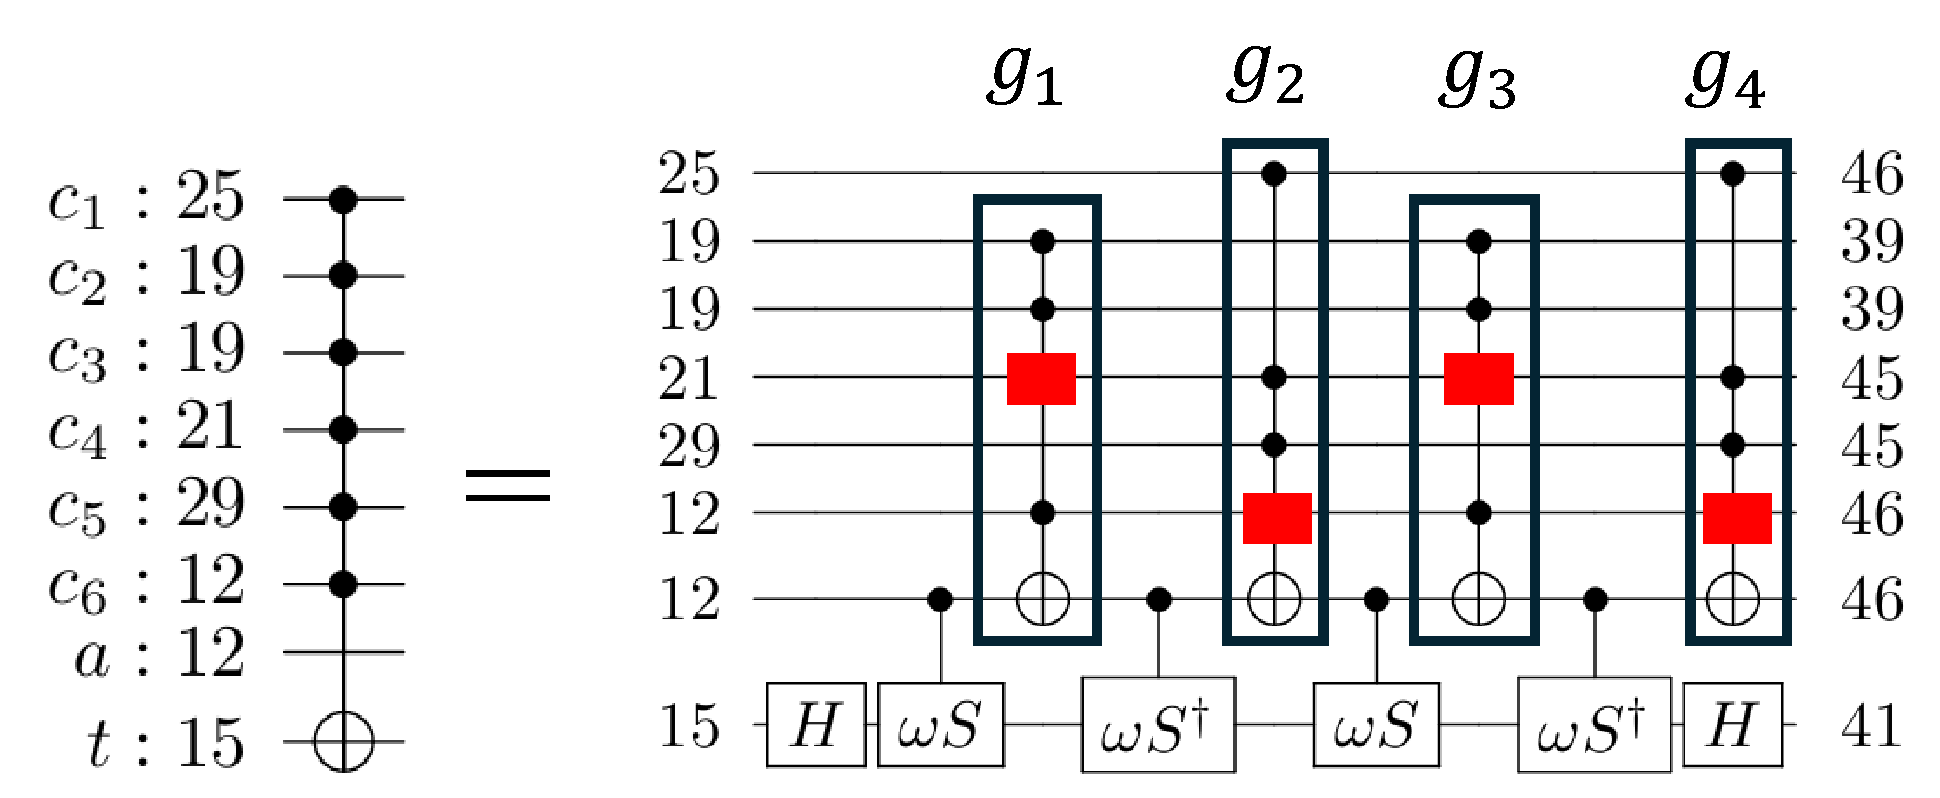
\includegraphics[width=10cm]{img/mimap_proposed.pdf}
  \caption{コントロールビット数が6個のMCTゲートをビットごとのT-depthを考慮し,手法~2を用いて分解した例}
  \label{mimap_proposed}
\end{figure}
\bout{図~\ref{mimap_proposed}にビットごとのT-depthを考慮し,
手法~2を用いて$c=6$のMCTゲートを4つのMCTゲートと,
4つの$C\omega S$ゲートに分解した例を示す.
まず,ビットごとのT-depthを考慮して,手法~2を用いてMCTゲートを分解するには,
式~\ref{eq:method2bunkatu}に従い,コントロールビットをT-depthの小さい順に2つの集合に分割する.
図~\ref{mimap_proposed}の例では,$C_{1}=\{c_{6}, c_{2},c_{3}\}, C_{2}=\{c_{1}, c_{4}, c_{5}\}$となる.
コントロールビットの分割を決定すると,
4つのMCTゲートと,$C\omega S$ゲートの構成するビットを決定できる.
図~\ref{mimap_proposed}の右側が,
$c=6$のMCTゲートを4つのMCTゲートと,
4つの$C\omega S$ゲートに分解した例である.}
\par
\bout{最後に,図~\ref{mimap_proposed}の右側の回路のゲートをAlgorithm~\ref{alg:method2_placement_decomp}
に従い分解する.
まず,$g_{1}$までのゲートの分解結果から各ビットのT-depthを計算し,
$c_{3}$を補助ビットとして用いて,$g_{1}$を分解する.
次に,$g_{2}$までのゲートの分解結果から,$c_{6}$を補助ビットとして用いて$g_{2}$を分解する.
最後に$g_{3}, g_{4}$は,それぞれ$g_{1}, g_{2}$の分解を逆変換に置換した上で,逆順にして配置する.
このようにして,各ゲートを分解することで,
図~\ref{mimap_proposed}の分解結果の最大のT-depthは46となる.}
\subsection{手法3}
手法~3にビットごとのT-depthを考慮した分解を適用する方法について説明する.
\par
手法~3では,分解に使用する値が不定の補助ビットの数$m\geq 2$と,
分解するMCTゲートのコントロールビット数$c$に応じて,
分解後の各MCTゲートのコントロールビット\rout{数を決定する.}
手法~3により求めた,
分解後の各MCTゲート$g_{1},\dots, g_{m+1}$の
コントロールビット数を$N_{1},\dots, N_{m+1}$とする.
ここで,手法~3では,
$1$番目と,$m+1$番目のゲートにコントロールビットを優先的に配置するため,
$N_{2},\dots, N_{m}$の値は2である.
\par
まず,手法~3の分解を決定するには,$g_{1},\dots ,g_{m+1}$の配置を決定する必要がある.
しかし,
$g_{1}$のコントロールビット数が3個以上であると,
$g_{1}$の分解の結果に応じて,$g_{2},\dots, g_{m+1}$で使用するビットのT-depthが変化する.
そのため,あらかじめ$g_{1}$をビットごとのT-depthを考慮し分解した上で,
その結果に応じて,$g_{2},\dots, g_{m+1}$の配置を決定する必要がある.
$g_{1},\dots,g_{m+1}$のコントロールビットの集合を$C_{1},\dots, C_{m+1}$とする.
分解に使用する値が$m$個の不定のビットの集合を$A$とする.
以下の手順に則り,$g_{1},\dots ,g_{m+1}$の配置を決定する.
\begin{enumerate}[手順1]
  \item $g_{1}$の配置を決定し,分解する.分解の結果から各ビットのT-depthを更新
  \begin{enumerate}
    \item $C_{1}$に$A$から,T-depthが最小の要素を移動する.
    \item $|C_{1}|=N_{1}$となるよう,$C$からT-depthが小さい順に要素を移動する.
    \item $t_{1}=t$とする.
    \item $C_{1}$と$t$でないビットのうちT-depthが小さい順に$|C_{1}|-2$個ビットを選択する.
    \item 選択したビットを補助ビットとして,ビットごとのT-depthを考慮し,手法~1で$g_{1}$を分解する.
    \item 分解の結果から,各ビットのT-depthを更新する.
  \end{enumerate}
  \item $g_{2}, \dots ,g_{m+1}$をT-depthが小さい順にビットを選択し,配置する.
  \begin{enumerate}[(1)]
    \item $i=2$とする.
    \item $C_{i}$に$A$のうち,T-depthが最小の要素を移動する.
    \item $|C_{i}|=N_{i}$となるよう,$C$からT-depthが小さい順に要素を移動する.
    \item $t_{i}$を$g_{i-1}$に移動した$A$の要素とする.
    \item $i < m+1$である限り,$i=i+1$とし,(2)に戻る.そうでなければ,終了する.
  \end{enumerate}
 \end{enumerate}
 このような手順で$g_{1},\dots ,g_{m+1}$の配置を決定する.
 その後,
 Algorithm~\ref{alg:method3_placement_decomp}に従い,
 分解とビットごとのT-depthの更新を繰り返し,
 数式~\ref{eq:bakerhaiti}の順番で並ぶMCTゲートを分解,配置する.
 \begin{algorithm}[tbp]
  \caption{ビットごとのT-depthを考慮した手法~3の配置と分解}
  \label{alg:method3_placement_decomp}
  \begin{algorithmic}[1]
    \Require 数式~\ref{eq:bakerhaiti}のMCTゲートのリスト:$mctlist$
    \Require 各ビットとT-depthの対応
    \Ensure 補助ビットを用いずClifford+Tに分解できるゲートで構成される回路:$OC$
    \ForEach{$g \leftarrow mctlist$}
    \State $g$で使用していないビットの集合:$A$
    \State $g$のコントロールビット数:$c$
    \State $A$からT-depthの小さい順にビットを$c-2$個取り出す.
    \State 取り出した$c-2$個のビットを補助ビットとして$g$をビットごとのT-depthを考慮し手法~1により分解
    \State $g$の分解結果を$OC$に追加,各ビットのT-depthを更新
    \EndFor
  \end{algorithmic}
\end{algorithm}
\par
\bout{図~\ref{baker_proposed}に,ビットごとのT-depthを考慮した手法~3により,$c=5$のMCTゲートを分解した例を示す.
図~\ref{baker_proposed}の分解について説明する.
まず,
手法~3を用いて,
図~\ref{baker_proposed}の左側のゲートを分解したときの,
各ゲートのコントロールビット数を求めると,
$N_{1}=3, N_{2}=2, N_{3}=2$となる.
次に,$g_{1}, g_{2}, g_{3}$を構成するビットを順に決定する.
まず,$g_{1}$のコントロールビット$C_{1}$を決定する.
補助ビット$a_{1}, a_{2}$のうち,T-depthが最小のビット$a_{2}$を$C_{1}$に移動する.
また,$c_{1},\dots,c_{5}$から,T-depthの値が小さい順に2つのビット,$c_{2}, c_{5}$を選択し,$C_{1}$に移動する.
$g_{1}$のターゲットビットを$t$とする.
$g_{1}$はコントロールビット数が3なので,$g_{1}$の分解結果により,後続のゲートを構成するビットが変化する.
そのため,$g_{1}$が使用していないビットから,T-depthが小さい順に$|C_{1}|-2$個ビットを選択し,$g_{1}$を分解する.
図~\ref{baker_proposed}の例では,$c_{3}$を補助ビットとし,$g_{1}$を分解し,T-depthを再計算する.
再計算すると,各ビットのT-depthは,$c_{2}=27, c_{3}=27, c_{5}=27, a_{2}=25, t=25$となる.
この結果から,$g_{2}, g_{3}$を構成するビットを決定する.
$g_{2}$のコントロールビットは$a_{1}$と,
$c_{1}, c_{3}, c_{4}$のうち,T-depthが最小のビットである$c_{1}$となる.
また,$g_{2}$のターゲットビットは,$a_{2}$となる.
$g_{3}$のコントロールビットは残りのコントロールビット$c_{3}, c_{4}$となり,
ターゲットビットは,$a_{1}$となる.
このようにして,$g_{1}, g_{2}, g_{3}$を構成するビットを決定し,
式~\ref{eq:bakerhaiti}の順で配置することで,図~\ref{baker_proposed}の右側の分解を実現できる.}
\par
\bout{最後に図~\ref{baker_proposed}
の右側のゲート$g_{1},\dots, g_{8}$を
Algrorithm~\ref{alg:method3_placement_decomp}に従い,
左側から分解,配置することで,ビットごとのT-depthを考慮した,手法~3の分解を決定できる.
まず,$g_{1}$はT-depth最小の$c_{3}$を補助ビットとして用いて分解する.
$g_{5}$は,$g_{1},\dots, g_{4}$の分解結果から,T-depth最小のビット$c_{4}$を補助ビットとして用いて分解する.
すべてのゲートを分解した結果,最大のT-depthは41となる.}
\begin{figure}[tbp]
  \centering
  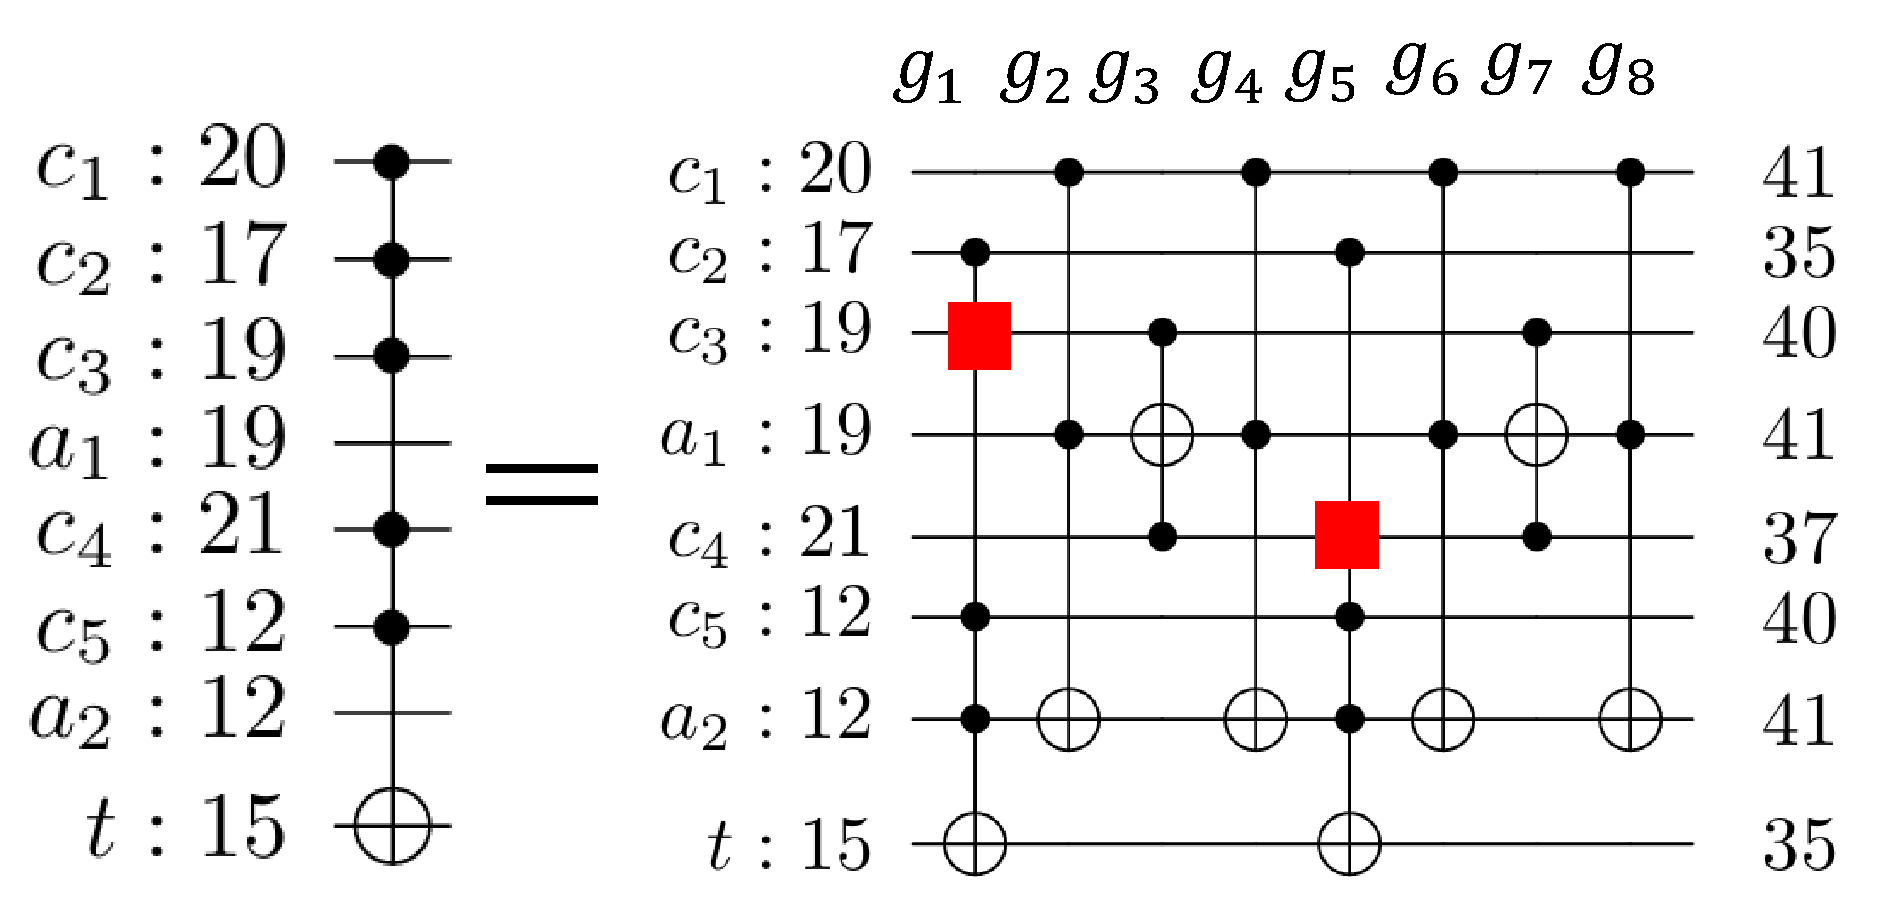
\includegraphics[width=10cm]{img/baker_proposed.pdf}
  \caption{2個の値が不定の補助ビットを用いて,ビットごとのT-depthを考慮し手法3を用いて,$c=5$のMCTゲートを分解した例}
  \label{baker_proposed}
\end{figure}
\begin{comment}
  \begin{algorithm}[tbp]
  \caption{ビットごとのT-depthを考慮した手法~3の配置と分解}
  \label{alg:method3_placement_decomp}
  \begin{algorithmic}[1]
    \Require 分解前のMCTゲート$(C, t)$ \Comment{$C$はコントロールビットの集合,$t$はターゲットビット}
    \Require $m$個の補助ビットのリスト$A$ 
    \Require 各ビットのT-depth
    \Ensure 補助ビットを用いずClifford+Tに分解できるゲートで構成される回路$OC$
    \State 空のビットのリスト$C_{1},\dots ,C_{m+1}$
    \State $m+1$個のビット$t_{1},\dots, t_{m+1}$
    \State $t_{1} \leftarrow t$
    \State $C_{1}$に$A$の内T-depthが最も小さいビットを追加
    \State $t_{2} \leftarrow A$の内T-depthが最も小さいビット
    \State $A$から最もT-depthが小さいビットを削除
    \State $C \leftarrow$ 分解前のMCTゲートのコントロールビット 
    \While{$|C_{1}|-2 \leq c+m-1$かつ$|C|\geq m$}
      \State $C_{1}$に$C$のT-depthが最も小さいビットを追加
      \State $C$の最もT-depthが小さいビットを削除
    \EndWhile
    \State $g_{1}\leftarrow (C_{1}, t_{1})$
    \State $g_{1}$を$g_{1}$を構成するビットでないビットのうち,$|C_{1}|-2$個のビットを使用し分解する
    \State $OC$に$g_{1}$の分解を追加
    \State 各ビットのT-depthを更新
    \For{$i={2,\dots ,m}$}
      \State $C_{i}$に$A$のT-depth最小の要素追加
      \State $t_{i+1}\leftarrow A$のT-depth最小の要素
      \State $A$からT-depth最小の要素を削除
      \State $C_{i}$に$C$のうち最もT-depthが小さな要素を追加
      \State $C$からT-depthが最も小さな要素を削除
      \State $g_{i}\leftarrow (C_{i}, t_{i})$
      \State $g_{i}$を$CCi\omega Z$ゲートに置換
      \State $OC$に$g_{i}$を追加
    \EndFor
    \State 各ビットのT-depthを更新
    \State $C_{m+1} \leftarrow C$
    \If{$|C_{m+1}|=2$}
    \State $g_{m+1}$を$CCiZ$ゲートに置換
    \State $g_{m+1}$を$OC$に追加
    \Else
    \State $g_{m+1}$を構成しないビットのうち,T-depthが小さい順に$|C_{m+1}|-2$個ビットを取り出す.
    \State 取り出したビットを補助ビットとして$g_{m+1}$をビットごとのT-depthを考慮し分解
    \EndIf
  \end{algorithmic}
\end{algorithm}
\end{comment}
\subsection{手法4}
手法4をビットごとのT-depthを考慮して分解する方法について説明する.
\par
手法4では,分解に使用する補助ビットの数に応じて,
複数段にMCTゲートを分解する.
分解した各MCTゲートのコントロールビット数は,
使用する補助ビットの数と,分解するMCTゲートのコントロールビット数に応じて,変化する.
分解に使用する値が不定の補助ビットの数を$d$,分解に使用する値が0の補助ビットの数を$k$とする.
これらの$c, k, d$の値により手法4から,
各段のMCTゲートのコントロールビット数が求められる.
手法4を用いて,
MCTゲートを分解したとき$n$段に分解できるとする.このとき,$n$は3以上の奇数である.
式~\ref{eq:niemann_cnt}のように,
2次元配列を用いて,求めた各段のMCTゲートのコントロールビット数を表すとする.
式~\ref{eq:niemann_cnt}では,
$n$段のゲートのうち,$\lceil \frac{n}{2} \rceil+1$段目以降のMCTゲートは,
1段目から$\lceil \frac{n}{2} \rceil -1$段目のゲートの複製であるため,省略している.
$N$の添え字は段数と何個目のMCTゲートであるかを表す.
例えば,$N_{i, j}$は,$i$段目$j$個目のMCTゲートのコントロールビット数を表す.
$\lceil \frac{n}{2} \rceil$段目は中心の段であるため,この段のゲート数は1個のみである.
そのため,$m_{\lceil \frac{n}{2} \rceil}=1$である.
\begin{equation}\label{eq:niemann_cnt}
  \begin{pmatrix}
    N_{1,1} & N_{1,2} & \dots & N_{1,m_{1}} \\
    N_{2,1} & N_{2,2} & \dots & N_{2,m_{2}} \\
    \vdots & \vdots & \ddots & \vdots \\
    N_{\lceil \frac{n}{2} \rceil,1} & N_{\lceil \frac{n}{2} \rceil,2} & \dots & N_{\lceil \frac{n}{2} \rceil,m_{\lceil \frac{n}{2} \rceil}}
  \end{pmatrix}
\end{equation}
この数式~\ref{eq:niemann_cnt}を用いて,図~\ref{niemann_c_2}の分解の各段のコントロールビット数を表したものを,
式~\ref{eq:niemann_c_2}に示す.
\begin{equation}\label{eq:niemann_c_2}
  \begin{pmatrix}
        2 & 2 & 2 & 2 \\
        2 & 2 &   & \\
        2 &   &   & \\
        2 &   &   & \\
  \end{pmatrix}
\end{equation}
\par
提案手法では,
手法~4により求めた各段のMCTゲートのコントロールビット数に従い,
分解後のMCTゲートの配置と分解を決定する.
分解に使用できる$k$個の値が0の補助ビットの集合を$CA$とする.
$\lceil \frac{n}{2} \rceil$段のMCTゲートを構成するビットは以下の手順で決める.
\begin{enumerate}[手順1]
  \item $i=1$とする.
  \item 空の集合$C_{1},\dots ,C_{m_{i}}$を用意する.$j=1$とする.
  \item $|C_{j}|=N_{i, j}$となるよう,$C$からT-depthが小さい順に要素を移動する.
  \item $j<m_{i}$であれば,$j=j+1$として手順3に戻る.
  \item $t_{1},\dots, t_{m_{i}}$に$CA$のT-depthが最小のビットを順番に一つずつ移動する.
  \item ゲート$g_{i, 1},\dots, g_{i, m_{i}}$のコントロールビットを$C_{1},\dots, C_{m_{i}}$とし,ターゲットビットを$t_{1},\dots ,t_{m_{i}}$とする.
  \item $g_{i, 1}, \dots ,g_{i, m_{i}}$で使用していないビットの集合$A$を求める.
  \item $k=1$とする.
  \item 同じ補助ビットを使わないよう,
  T-depthが小さい順に$A$から$|C_{m_{k}}-2|$個補助ビットを選択し,$A$からそれらの要素を削除する.
  \item 選択した補助ビットを用いて,
  ビットごとのT-depthを考慮し,$g_{i, k}$を手法1で分解する.
  \item $k < m_{i}$であれば,$k=k+1$して,手順9に戻る.そうでなければ次に進む.
  \item 各ビットのT-depthを更新する.
  \item $C$に$t_{1},\dots, t_{m_{i}}$を追加する.
  \item $i< \lceil \frac{n}{2} \rceil$であれば,$i=i+1$とし,手順2に戻る.
  \item MCTゲート$g_{\lceil \frac{n}{2} \rceil, 1}$のコントロールビットを$C$,ターゲットビットを$t$とする.
\end{enumerate}
以上の手順で,$1,\dots ,\lceil \frac{n}{2} \rceil$段のMCTゲートを構成するビットを決定する.
構成するビットを決定した各段のMCTゲートは式~\ref{eq:niemann_gates}のような形で複製を含め情報をもつ.
\begin{equation}\label{eq:niemann_gates}
  \begin{pmatrix}
    g_{1,1} & g_{1,2} & \dots & g_{1,m_{1}} \\
    g_{2,1} & g_{2,2} & \dots & g_{2,m_{2}} \\
    \vdots & \vdots & \ddots & \vdots \\
    g_{\lceil \frac{n}{2} \rceil,1} & g_{\lceil \frac{n}{2} \rceil,2} & \dots & g_{\lceil \frac{n}{2} \rceil,m_{\lceil \frac{n}{2} \rceil}}\\
    g_{\lceil \frac{n}{2} \rceil -1, 1} & g_{\lceil \frac{n}{2}  \rceil-1 ,2}& \dots & g_{\lceil \frac{n}{2} \rceil-1 ,m_{\lceil \frac{n}{2} \rceil-1}}\\
    \vdots & \vdots & \ddots &\vdots \\
    g_{1,1} & g_{1,2} & \dots & g_{1,m_{1}} \\
  \end{pmatrix}
\end{equation}
\par
構成するビットを決定した,
数式~\ref{eq:niemann_gates}の
MCTゲートをそれぞれビットごとの
T-depthを考慮し手法1を用いて分解することで,
手法4の分解は決定できる.
Algorithm~\ref{alg:method4_placement_decomp}に従い,
数式~\ref{eq:niemann_gates}の
MCTゲートの分解と配置を繰り返し,分解を決定する.
\begin{algorithm}[tbp]
  \caption{ビットごとのT-depthを考慮した手法~4の分解と配置}
  \label{alg:method4_placement_decomp}
  \begin{algorithmic}[1]
    \Require 数式~\ref{eq:niemann_gates}のMCTゲートの2次元配列:$mctlist$
    \Require 各ビットとT-depthの対応
    \Ensure 補助ビットを用いずClifford+Tに分解できるゲートで構成される回路:$OC$
    \ForEach{$pqgate \leftarrow mctlist$}
    \State $pqgate$で使用していないビットの集合:$A$
    \ForEach{$g\leftarrow pqgate$}
      \State $g$のコントロールビット数:$c$
      \State $A$からT-depthの小さい順にビットを$c-2$個取り出す.
      \State $A$から,取り出した$c-2$個のビットを削除.
      \State 取り出した$c-2$個のビットを補助ビットとして$g$をビットごとのT-depthを考慮し手法~1により分解
      \State $g$の分解結果を$OC$に追加
    \EndFor
      \State 各ビットのT-depthを更新
    \EndFor
  \end{algorithmic}
\end{algorithm}
\par
\begin{figure}
  \centering
  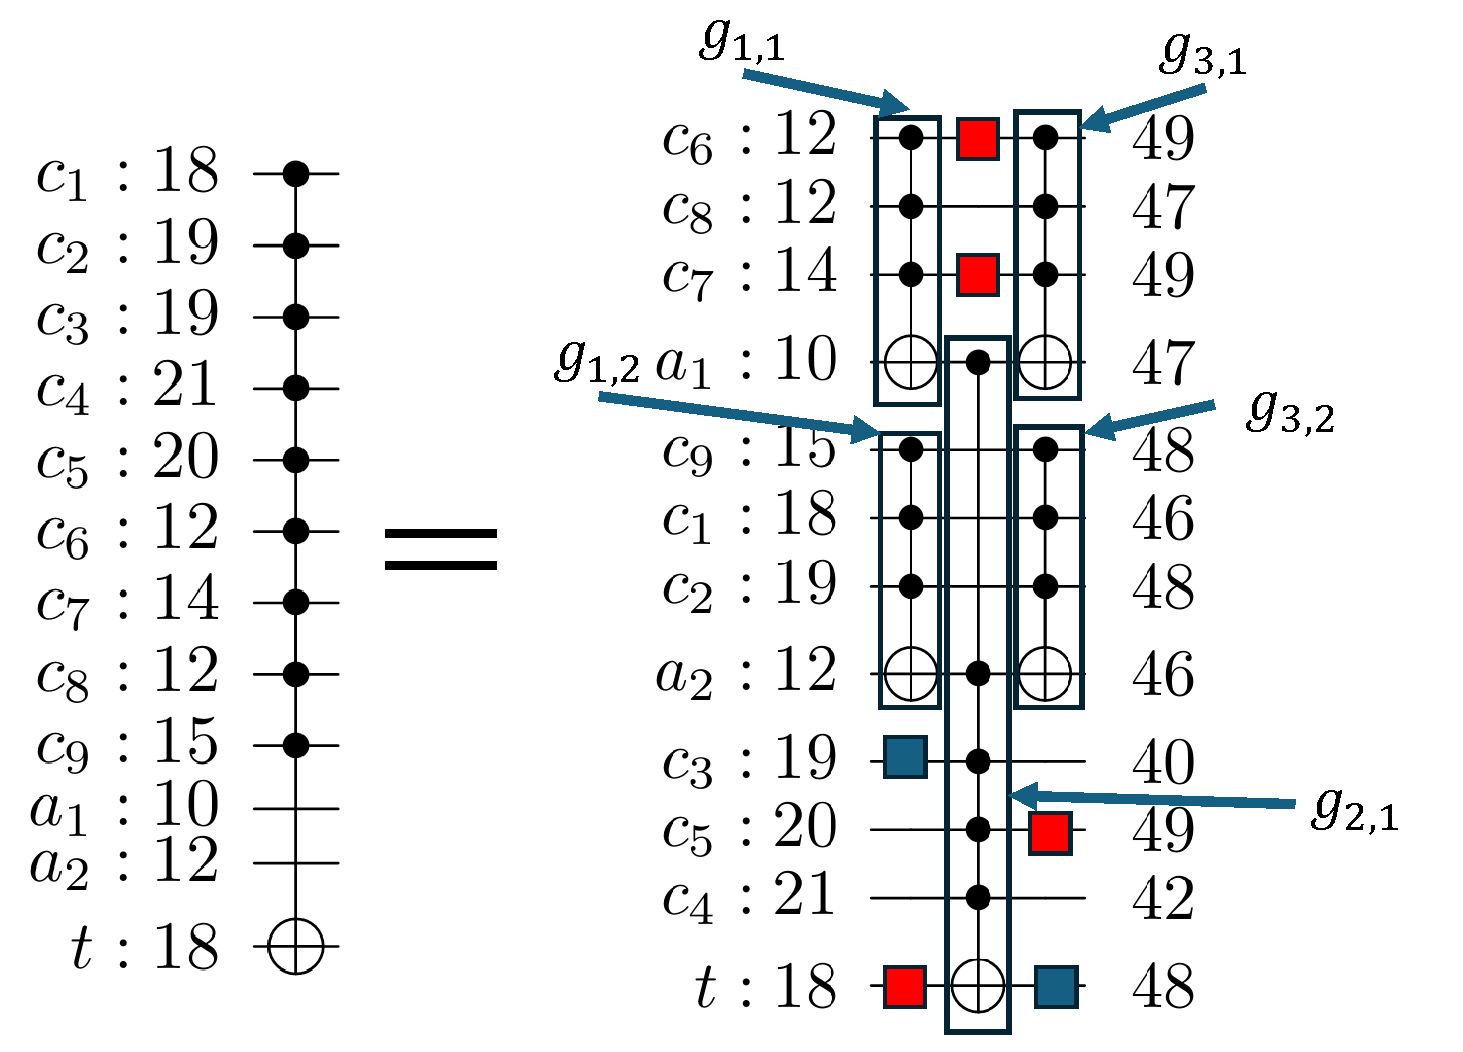
\includegraphics[width=10cm]{img/niemann_proposed.pdf}
  \caption{2個の値が0の補助ビットを用いて,ビットごとのT-depthを考慮し手法4を用いて,$c=9$のMCTゲートを分解した例}
  \label{niemann_proposed}
\end{figure}
\bout{図~\ref{niemann_proposed}に2個の値が0の補助ビットを用いて,
ビットごとのT-depthを考慮した手法~4で$c=9$のMCTゲートを分解した例を示す.
図~\ref{niemann_proposed}では,
分解前のMCTゲートのコントロールビットは$C=\{c_{1},\dots, c_{9}\}$となり,ターゲットビットは$t$である.
また,値が0の補助ビットは$CA=\{a_{1}, a_{2}\}$である.
まず,手法~4により各段のMCTゲートのコントロールビット数を求めると,式~\ref{eq:niemann_ctrl_gutairei}のようになる.
\begin{equation}\label{eq:niemann_ctrl_gutairei}
  \begin{pmatrix}
    3 & 3  \\
    5 &    \\
\end{pmatrix}
\end{equation}
この求めた数式~\ref{eq:niemann_ctrl_gutairei}のコントロールビット数に従い,各ゲートを構成するビットを決定する.
まず,1~段目のゲート$g_{1,1}, g_{1,2}$を構成するビットを決定する.
T-depthの小さい順にコントロールビットを$C$から選択すると,
1段目のゲートのコントロールビットは,それぞれ,$C_{1,1}=\{c_{6}, c_{8}, c_{7}\}$と,$C_{1,2}=\{c_{9}, c_{1}, c_{2}\}$となる.
選択したコントロールビットは$C$から削除する.
次に1段目のゲートのターゲットビットは,T-depthが小さい順に選択すると,それぞれ$a_{1}$, $a_{2}$となる.
選択した値が0の補助ビットは,$C$に追加し,$CA$から削除する.
1段目のゲート$g_{1,1},g_{1,2}$を構成するビットを決定した後,
$g_{1,1}, g_{1,2}$で使用していないビットの集合$A$を求める.
このとき,$A=\{c_{3}, c_{5}, c_{4}, t\}$となる.
このビットのうち,T-depthが小さい順に$c_{3},c_{5}$を補助ビットとして使用し,$g_{1,1}, g_{1,2}$を分解して,T-depthを更新する.
次に,2段目のゲート$g_{2,1}$を構成するビットを決定する.
2段目のゲートは中心のゲートであるため,
コントロールビットは残りの$C=\{a_{1},a_{2}, c_{3},c_{5}, c_{4}\}$となり,
ターゲットビットは$t$となる.
このようにして,$g_{1,1}, g_{1,2}, g_{2,1}$の構成するビットを決定する.
これらのゲートを構成するビットを決定した後,
式~\ref{eq:niemann_gates}の順でMCTゲートを配置すると,
図~\ref{niemann_proposed}の右側の分解となる.}
\par
\bout{最後に,図~\ref{niemann_proposed}の右側のゲートを
Algorithm~\ref{alg:method4_placement_decomp}に従い,分解する.
まず,1段目のゲート$g_{1,1}, g_{1,2}$を分解する.
$g_{1,1}$は赤色で塗りつぶされたビット$t$を補助ビットとして使用し分解する.
$g_{1,2}$は青色で塗りつぶされたビット$c_{3}$を補助ビットとして使用し分解する.
次に,$g_{1,1},g_{1,2}$の分解の結果から,
赤色で塗りつぶされたビット$c_{6},c_{7}$を補助ビットとして使用し,$g_{2,1}$を分解する.
最後に,$g_{2,1}$の分解の結果から,
$g_{3,1}, g_{3,2}$はそれぞれ,$c_{5}, t$を補助ビットとして使用し分解する.
このようにして,全てのゲートを分解すると,最大のT-depthは49となる.}
% どの補助ビットを選択したか図に書く.
\begin{comment}
提案手法では,
手法4により求めた各段のMCTゲートのコントロールビット数に従い,
分解後のMCTゲートの配置と分解を決定する.
Algorithm~\ref{}に各段のMCTゲートの配置,分解の決定方法を示す.
\begin{algorithm}[tbp]
  \caption{ビットごとのT-depthを考慮した手法~3の配置と分解}
  \label{alg:method3_placement_decomp}
  \begin{algorithmic}[1]
    \Require 分解前のMCTゲート$g=(C,t)$
    \Require 手法4で求めた各段のMCTゲートのコントロールビット数を表す2次元配列$CntList$
    \Require 値が0のビットのリスト$CA$
    \Require 値が不定のビットのリスト$DA$
    \Require 各ビットのT-depth
    \Ensure 分解後の回路$OC$
    \ForEach{$v$ in $CntList$}
    \State $n$:$v$の要素数
    \State $g_{1},\dots, g_{n}$:配置を行うMCTゲート
    \State $C_{1},\dots ,C_{n}$:各MCTゲートのコントロールビットの集合
    \State $t_{1},\dots ,t_{n}$:各MCTゲートのターゲットビット
    \ForEach{$c$ in $v$ with index $i$}
    \For{$j=1$ to $c$}
    \State $C_{i}$に$C$のT-depthが最も小さいビットを追加
    \State $C$からT-depthが最も小さいビットを削除
    \EndFor
    \State $t_{i}$に$CA$のT-depthが最も小さいビットを追加
    \State $CA$からT-depthが最も小さいビットを削除
    \EndFor
    \State $g_{1},\dots ,g_{n}$を同じ補助ビットを使わないよう,ビットごとのT-depthを考慮し分解
    \State $OC$に$g_{1},\dots g_{n}$の分解を追加
    \State T-depthを再計算
    \State $t_{1},\dots, t_{n}$を$C$に追加
    \EndFor
  \end{algorithmic}
\end{algorithm}
\end{comment}
\section{逆順での分解}
本節では,MCTゲートを逆順で分解する場合について説明する.
\begin{figure}[tbp]
  \centering
  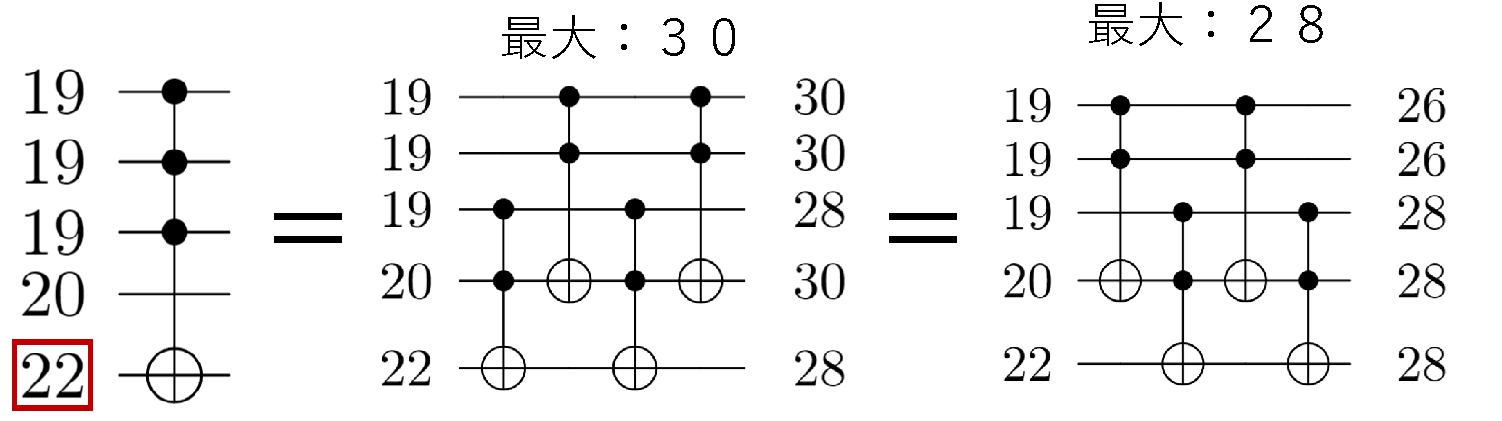
\includegraphics[width=10cm]{img/reverse_mct.pdf}
  \caption{コントロールビット数が3個のMCTゲートの分解とその逆順の分解}
  \label{reverse}
\end{figure}
\par
図~\ref{reverse}に示すように,
分解に使用する補助ビットと,分解するMCTゲートを構成するビットの中で,
ターゲットビットのT-depthが最も大きい場合,
MCTゲートを逆順で分解することで,
T-depthを削減できる.
図~\ref{reverse}の中心の分解は,
左側のMCTゲートを手法1の順で分解した場合を示している.
一方で右側の分解は,
左側のMCTゲートを手法1の分解と逆順に分解した場合を示している.
中心の例の分解では,
必ず最も左側のMCTゲートでターゲットビットを使用するため,
T-depthを削減することができない.
このため,
ターゲットビットのT-depthが最も大きい場合,逆順で分解することでT-depthを削減できる.
図~\ref{reverse}の例では,逆順でMCTゲートを分解することで最大のT-depthを2,削減している.
\par
手法1を用いて,MCTゲートを逆順で分解するには,
式~\ref{eq:toffoli_haiti}の逆順で配置する必要がある.
そのため,
$g_{2},\dots ,g_{c-1}, g_{1}$の順に優先的にT-depthが小さいビットを使用する必要がある.
分解前のMCTゲートの$c$個のコントロールビットを
T-depthが小さい順に並び変えたものを$c_{1},\dots, c_{c}$とする.
$g_{1},\dots, g_{c-1}$のコントロールビットの集合を$C_{1},\dots, C_{c-1}$とする.
$c-2$個の値が不定の補助ビットをT-depthの小さい順に並び変えたものを,$a_{1},\dots ,a_{c-2}$とする.
$g_{1},\dots ,g_{c-1}$の構成するビットの決定方法を以下に示す.
\begin{enumerate}[手順1]
  \item $g_{2}$のターゲットビットを$a_{1}$とする.
  \item $C_{2}\dots, C_{c-2}, C_{1}$に$a_{2},\dots, a_{c-2}, a_{1}$をそれぞれ順番に1つずつ追加する.
  \item $C_{2},\dots ,C_{c-2}$に順番に$c_{1},\dots ,c_{c-3}$を追加する.
  \item $C_{c-1}$に$c_{c-2}, c_{c-1}$を追加する.
  \item $C_{1}$に$c_{c}$と$a_{1}$を追加する.
  \item $g_{3},\dots, g_{c-2}$のターゲットビットをそれぞれ順番\rout{に}$a_{2}, \dots , a_{c-3}$とする.
  \item $g_{1}$のターゲットビットを$t$とする.
\end{enumerate}
$g_{1},\dots, g_{c-1}$の構成するビットを決定後,
式~\ref{eq:toffoli_haiti}の逆の順番で配置を行うことで,逆順で手法1の分解ができる.
\par
手法~2についても,逆順で分解することで,ターゲットビットを\bout{後で}使用できる.
配置する4つのMCTゲート$g_{1},\dots, g_{4}$と4つの$C\omega S$ゲートを逆順で配置することで,逆順の分解ができる.
分解に使用する1つの値が不定のビットを$a$とする.
4つの$C\omega S$ゲートは逆順で分解しても変わらず$a$をコントロールビットにもち,$t$をターゲットビットに持つ.
逆順で分解する場合$g_{4},\dots, g_{1}$の順で左側からMCTゲートを配置するため,
$g_{4}, g_{2}$にT-depthの小さいビットを配置する必要がある.
そのため,$g_{1}, g_{2}$のコントロールビットの集合を$C_{2}, C_{1}$として,
式~\ref{eq:method2bunkatu}の通りに$C_{1}, C_{2}$を決定する.
各ゲートを構成するビットを決定したら,
$g_{4}, C\omega S, g_{3}, C\omega S, \dots , g_{1}, C\omega S$の順で分解と配置を繰り返せば,
手法~2の逆順での分解を実現できる.
\par
手法3を逆順で分解するには,
式~\ref{eq:bakerhaiti}の逆順で分解したMCTゲートを配置する必要がある.
そのため,$g_{2},\dots, g_{m+1}, g_{1}$の順でT-depthの小さいビットを配置する必要がある.
分解に用いる$m$個の補助ビットの集合を$A$とする.
手法~3により求めた,
分解後の各MCTゲート$g_{1},\dots, g_{m+1}$の
コントロールビット数を$N_{1},\dots, N_{m+1}$とする.
$g_{1},\dots,g_{m+1}$のコントロールビットの集合を$C_{1},\dots, C_{m+1}$とする.
$g_{1},\dots,g_{m+1}$のターゲットビットを$t_{1},\dots, t_{m+1}$とする.
以下の手順に則り,$g_{1},\dots ,g_{m+1}$を構成するビットを決定する.
\begin{enumerate}[手順1]
  \item $g_{2}$を構成するビットを決定する.
  \begin{enumerate}
    \item $C_{2}$に$A$の最もT-depthが小さい要素を移動する.
    \item $t_{2}$に$A$の最もT-depthが小さい要素を移動する.
    \item $g_{2}$に$C$の最もT-depthが小さい要素を移動する.
  \end{enumerate}
  \item $g_{3},\dots, g_{m+1}$を構成するビットを決定する.
  \begin{enumerate}
    \item $i=3$とする.
    \item $C_{i}$に$A$から,T-depthが最小の要素を移動する.
    \item $|C_{i}|=N_{i}$となるよう,$C$からT-depthが小さい順に要素を移動する.
    \item $t_{i}$を$C_{i-1}$に移動した$A$の要素とする.
  \end{enumerate}
  \item $g_{1}$を構成するビットを決定する.
  \begin{enumerate}
    \item $C_{1}$に$t_{2}$を加える.
    \item $C_{1}$に,$C$の残りの要素を移動する.
    \item $t_{1}$を$t$とする.
  \end{enumerate}
 \end{enumerate}
 このような手順で$g_{1},\dots ,g_{m+1}$を構成するビットを決定し,式~\ref{eq:bakerhaiti}の逆の順でゲートを配置,
 分解することで,手法3についても逆順で分解できる.
 \par
 手法4については,分解が左右対称であるため,逆順で分解してもT-depthに変化がない.
% 手法2,3個別に説明をいれる.
\section{\bout{後続}のゲートを考慮した\bout{ビームサーチによる分解手法}}
後続のゲートを考慮し,\bout{ビームサーチによってMCTゲートの分解を行う手法を説明する.}
\par
図~\ref{select_ancilla_tdepth}に,
2つのMCTゲート$g_{1}, g_{2}$の補助ビットの選択によるT-depthの変化を示す.
図~\ref{select_ancilla_tdepth}の\bout{真ん中}の例は,
$g_{1}$が赤で塗りつぶされたT-depth最小の補助ビットを選択し分解,
$g_{2}$が$g_{1}$の分解の結果を受けて,青で塗りつぶされたT-depth最小のビットを選択し,分解した例である.
図~\ref{select_ancilla_tdepth}の右側の例では,
$g_{1}$が赤で塗りつぶされたT-depthが41の補助ビットを選択し,分解,
$g_{2}$が$g_{1}$の分解の結果を受けて,
青で塗りつぶされた,T-depth最小のビットを選択した例である.
図~\ref{select_ancilla_tdepth}中心の例では,
最大のT-depthが58となるのに対し,
右側の例では,最大のT-depthが53となる.
\begin{figure}[tbp]
  \centering
  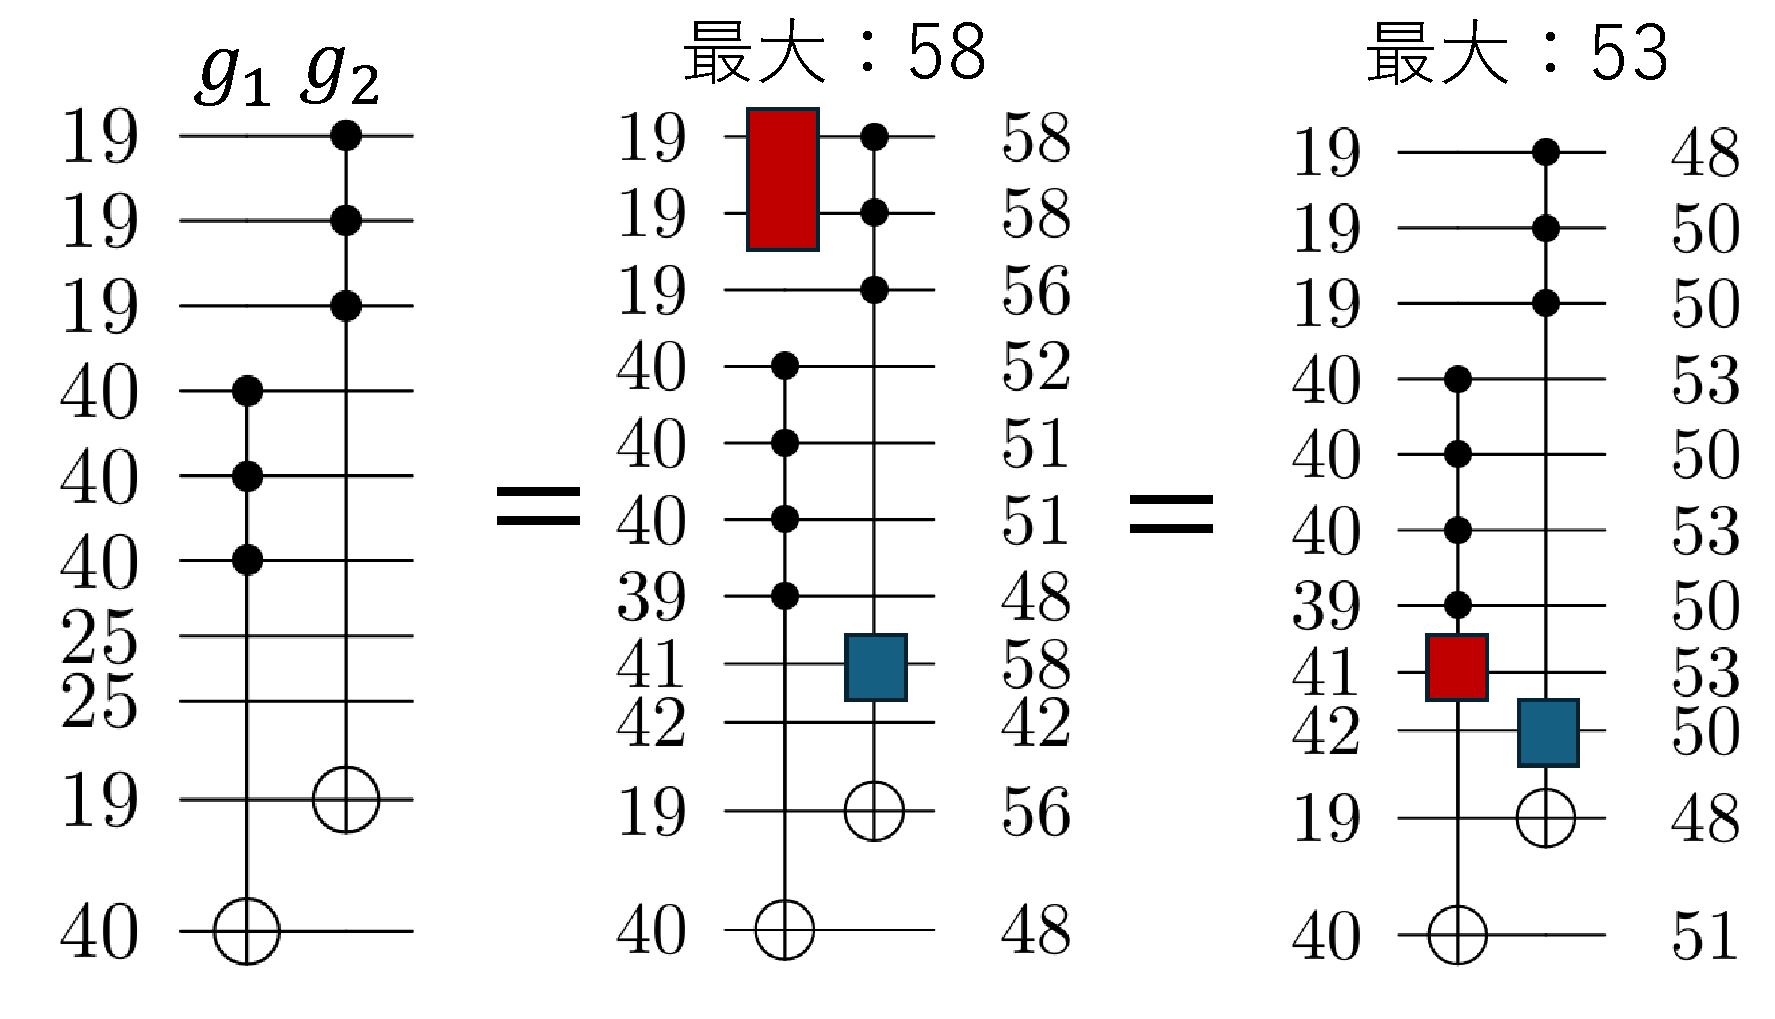
\includegraphics[width=10cm]{img/select_ancilla_biit_tdepth.pdf}
  \caption{2つのMCTゲートの補助ビットの選択によるT-depthの変化の例}
  \label{select_ancilla_tdepth}
\end{figure}
図~\ref{bad_consider_tdepth}の中心の例のように,
貪欲にT-depthの小さいビットを選択した場合,
\bout{後続}のゲートを分解した場合にT-depthが悪化する場合がある.
このため,分解するゲートの\bout{後続}のゲートを考慮しMCTゲートを分解することが必要である.
\par
ビットごとのT-depthを考慮したMCTゲートの分解を行う場合,
MCTゲートの分解の結果に応じて各ビットのT-depthが変化する.
そこで,各ノードの評価値をT-depthの最大値とし,
各MCTゲートの分解を遷移とし,木を構成する.
この木を全探索することで,最適な分解を求めることができる.
しかし,全探索を行うと量子ビット数と,
分解を行うMCTゲート数が増加すると計算量が膨大になる.
このため,ビームサーチ\cite{bisiani1992beam}を用い,
探索範囲を事前に決めておいた数の候補に限定することで,
現実的な計算量に抑えて,探索を行う.
\par
ここで,各MCTゲートの分解の列挙も制限する.
すべての分解を列挙するには,すべての補助ビットの選択の組み合わせを列挙しなければならない.
コントロールビット数が$c$のMCTゲートは,$1$から$c-2$個の値が不定の補助ビットを選択できる.
使用できる値が不定の補助ビットの数が$m$とすると,
値が不定の補助ビットの選び方は,$\sum_{i = 1}^{c-2} {}_mC_{i}$通りとなる.
回路の量子ビット数と回路を構成するMCTゲートのコントロールビット数が増加すると,
補助ビットの選択をすべて列挙することは難しいため,
規定した分解を遷移として,遷移の数を制限する.
規定した分解は次の通りである.
\begin{enumerate}[(1)]
  \item T-depthが小さい順に1から$c-2$個の値が不定の補助ビットを選択
  \item T-depthが小さい順に1から$c-2$個の値が0の補助ビットを選択
  \item 分解を行うゲートの一つ後のゲートが使用していないビットを,値が不定のビットとして,T-depthが小さい順に1から$c-2$個選択する.
  \item これらの分解の逆順の分解
\end{enumerate}
\par
MCTゲートの分解を遷移とし,分解を行った後のT-depthの最大値を評価値として,
ビームサーチを行う疑似コードをAlgorithm~\ref{alg:mct_beam}に示す.
図~\ref{mct_beam}に,
図~\ref{select_ancilla_tdepth}の$g_{1}$の分解を
Algorithm~\ref{alg:mct_beam}に従い,
決定する様子を示す.
図~\ref{mct_beam}の探索する幅は3,探索する深さは2とする.
また,簡単のため,逆順の分解については列挙しない.
まず,図~\ref{mct_beam}では,
$g_{1}$の分解\rout{$D_{1},\dots, D_{4}$を列挙する.}
分解$D_{1},\dots,D_{4}$から求まる回路の最大のT-depthをノードの評価値とする.
評価値の小さい順にノードをソートし,
上位3つのノードから,次のゲート$g_{2}$の分解を列挙する.
$g_{2}$の分解の結果からT-depthを計算し,
評価値が最小のノードの最初の遷移を$g_{1}$の分解として決定する.
この例では,$D_{3}$が$g_{1}$の分解として決定する.
\begin{figure}[tbp]
  \centering
  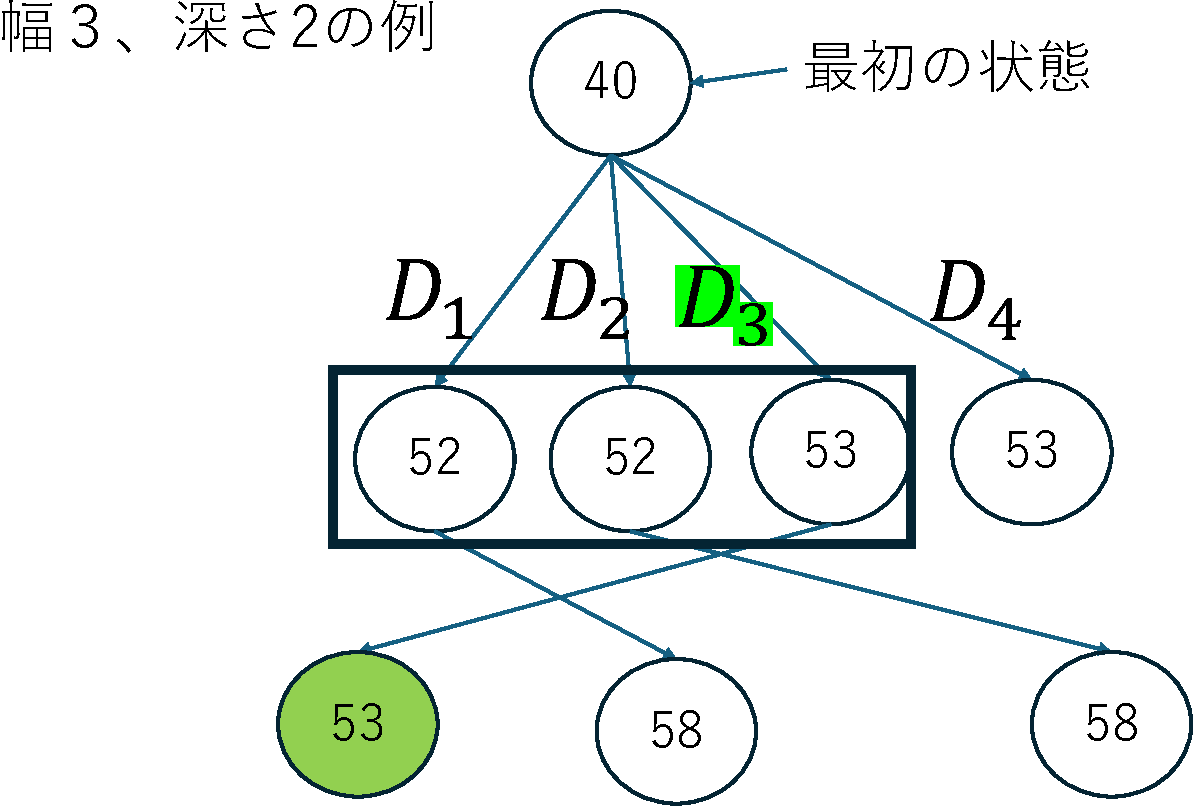
\includegraphics[width=8cm]{img/mct_beam.pdf}
  \caption{図~\ref{select_ancilla_tdepth}の$g_{1}$の分解をAlgorithm~\ref{alg:mct_beam}に従い決定するようす}
  \label{mct_beam}
\end{figure}
提案手法では,MCTゲートで構成される回路に対して,1ゲートずつ,
Algrorithm~\ref{alg:mct_beam}に基づいて分解を決定していき,すべてのゲートを分解する.
% 具体例を付けるべきか,図の例だと大した例にならない.
\begin{comment}
図~\ref{mct_beam}に探索する深さ2,幅3でビームサーチを用いて,
図~\ref{bad_consider_tdepth}を後のゲートを考慮しMCTゲートの分解を決定する様子を示す.
\begin{figure}[tbp]
  \centering
  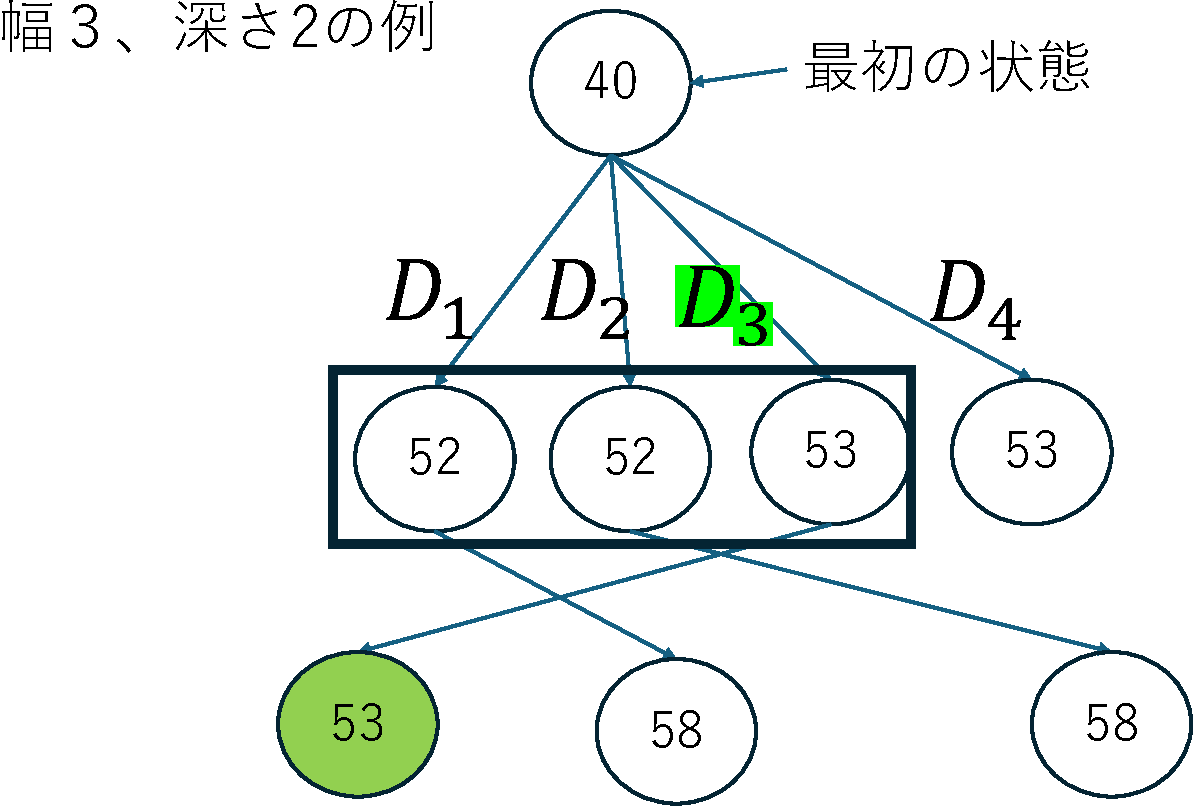
\includegraphics[width=10cm]{img/mct_beam.pdf}
  \caption{2つのMCTゲートの補助ビットの選択によるT-depthの変化の例}
  \label{mct_beam}
\end{figure}
\end{comment}

\begin{algorithm}[tbp]
  \caption{T-depthの最大値を評価値とするビームサーチの疑似コード}
  \label{alg:mct_beam}
  \begin{algorithmic}[1]
    \Require $state$:(T-depthの最大値,ビットごとのT-depth,分解を行うMCTゲート)
    \Require $legal\_actions$:MCTゲートの分解を列挙し,次のゲート分解前の状態を返す関数
    \Require $depth$:探索する深さ
    \Require $width$:探索する幅
    \State $best\_decomp$:最良の候補
    \State $candidate\_list$ 探索候補のリスト,優先度付きキュー
    \State $candidate\_list.push(state)$
    \For{$1,..,depth$}
      \State $next\_candidate\_list$ 次の探索候補のリスト,優先度付きキュー
      \For{$1,..,width$}
      \If{$candidate\_list$が空なら}
        \State break
      \EndIf
      \State $now\_state \Leftarrow candidate\_list.pop()$ 探索候補の最良の値を取り出し,popする
      \State $next\_candidate\_list.push(legal\_actions(now\_state))$ 次の探索候補のリストに現在の状態からの遷移を追加
      \EndFor
      \State $candidate\_list \Leftarrow next\_candidate\_list$ 探索候補のリストを更新
      \State $best\_decomp \Leftarrow candidate\_list.top()$ 最良の候補を更新
    \EndFor
    \State \Return $best\_decomp$の最初の遷移を返す
  \end{algorithmic}
\end{algorithm}
